\section{Domain Model}
\label{sec:model}

After defining the fundamental concepts of the domain, it is important to underline which relationship they have. The following diagrams show the different types of relationship that define the domain's model.

The figure \ref{fig:domain-overview} shows the principal elements of a \textit{Micro City}. In particular, a \textit{Micro City} is composed of many guests that may benefit from activities inside it. Each guest owns a wearable device that allows to interact with the \textit{Micro City}. Many guests moving together compose a group of guests. An activity may give rewards to guests (or group of guests) that follow recommendations.

\begin{figure}[H]
    \centering
    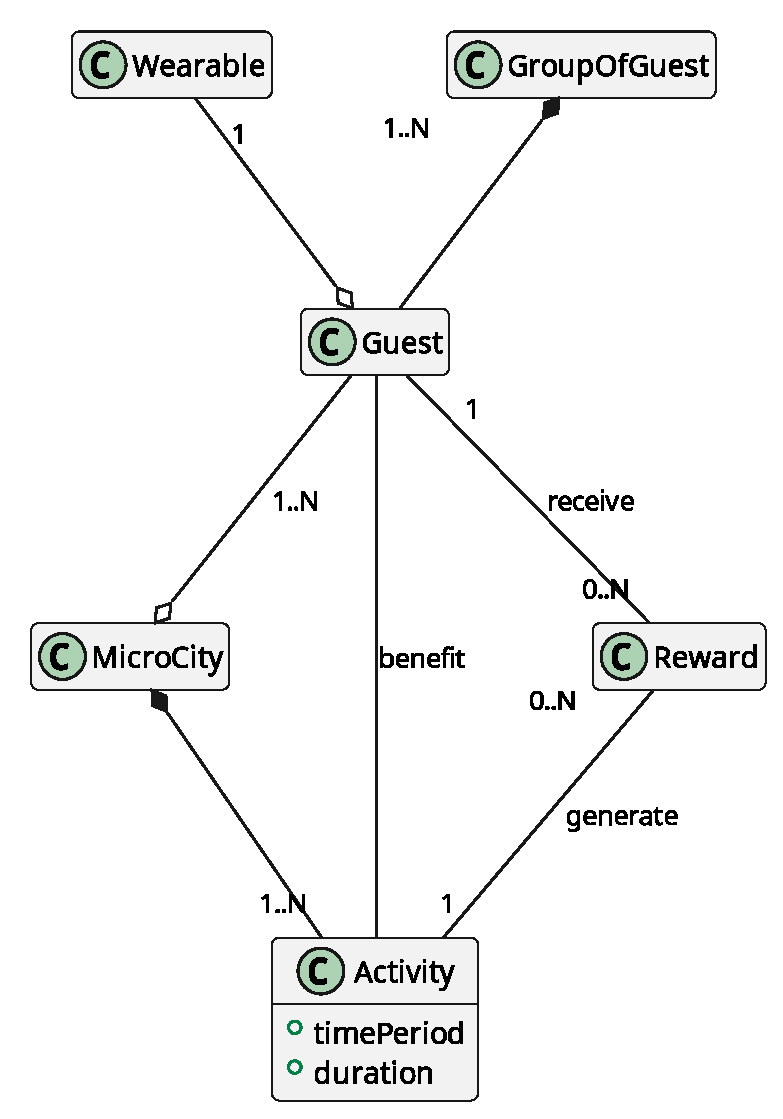
\includegraphics[width=0.55\textwidth]{./img/domain_overview-0}
    \caption{Class diagram of the \textit{Micro City}'s domain model.}
    \label{fig:domain-overview}
\end{figure}

\newpage

The figure \ref{fig:micro-city} shows a diagram representing a \textit{Micro City}'s organization. A \textit{Micro City} has a map and many workers. Both the activities and the \textit{Micro City} may request the payment of a fee, that is a certain amount of money in order to access to them. There are two types of activities: services, that are continuously available during a \textit{Micro City}'s lifetime, and events, that takes place in a specific moment and has a limited duration. A queue represents the waiting time before that a guest can benefit from an activity.

\begin{figure}[H]
    \centering
    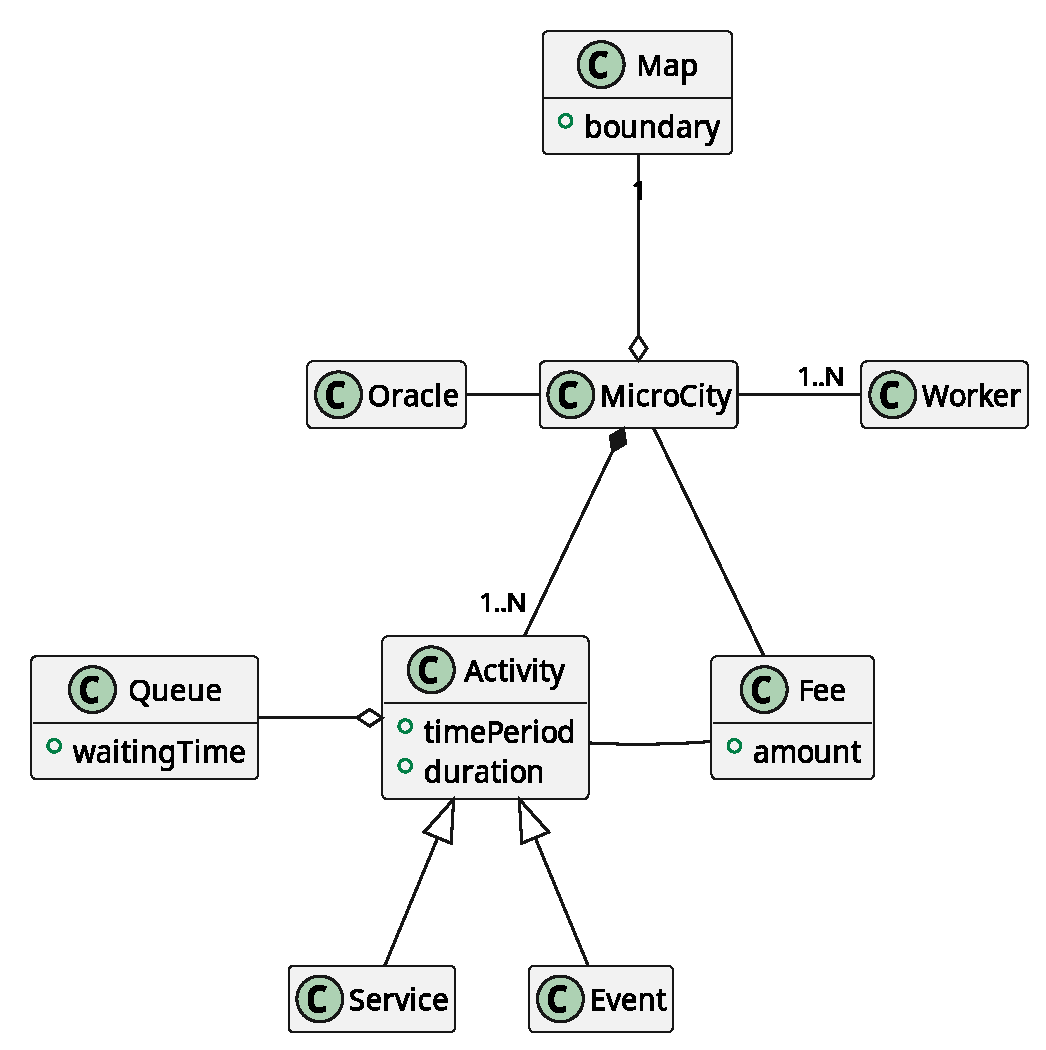
\includegraphics[width=0.7\textwidth]{./img/micro_city-0}
    \caption{Class diagram that models the organization of a \textit{Micro City}.}
    \label{fig:micro-city}
\end{figure}

\newpage

The figure \ref{fig:reward} shows the sequence diagram that explains how a guest can obtain a reward.

\begin{figure}[H]
    \centering
    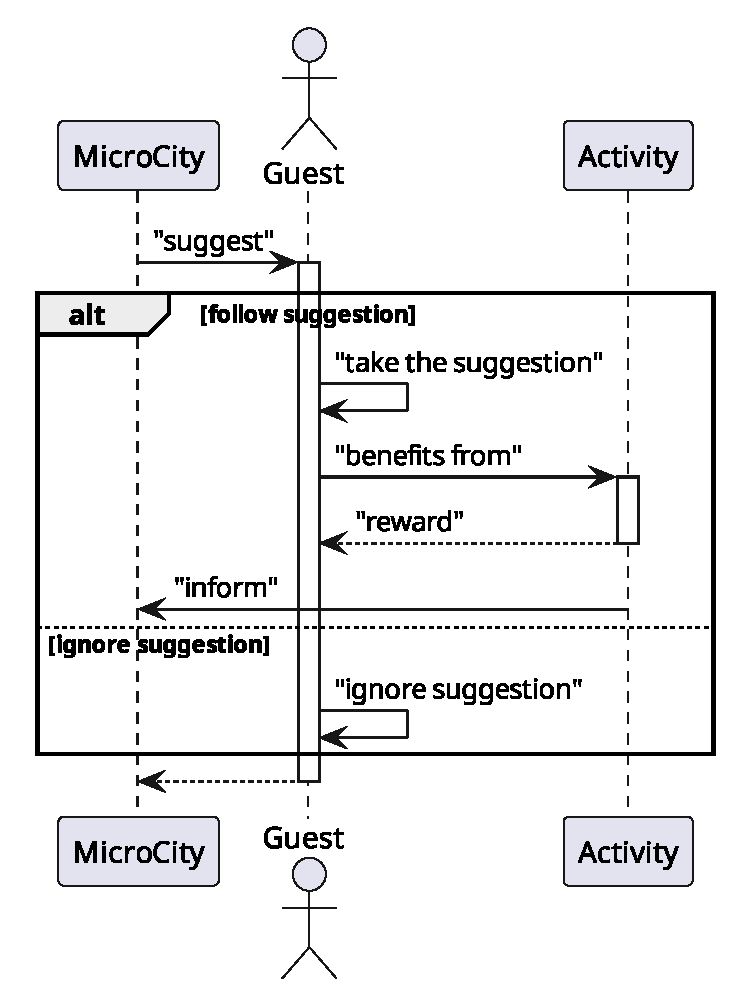
\includegraphics[width=0.6\textwidth]{./img/reward-0}
    \caption{Sequence diagram that shows how to obtain a reward.}
    \label{fig:reward}
\end{figure}

\newpage
